	\documentclass[10pt,oneside]{CBFT_book}
	% Algunos paquetes
	\usepackage{amssymb}
	\usepackage{amsmath}
	\usepackage{graphicx}
	\usepackage{libertine}
% 	\usepackage[bold-style=TeX]{unicode-math}
	\usepackage{lipsum}

	\usepackage{natbib}
	\setcitestyle{square}

	\usepackage{polyglossia}
	\setdefaultlanguage{spanish}


	\usepackage{CBFT.estilo} % Cargo la hoja de estilo

	% Tipografías
	% \setromanfont[Mapping=tex-text]{Linux Libertine O}
	% \setsansfont[Mapping=tex-text]{DejaVu Sans}
	% \setmonofont[Mapping=tex-text]{DejaVu Sans Mono}

	%===================================================================
	%	DOCUMENTO PROPIAMENTE DICHO
	%===================================================================

\begin{document}

\chapter{Pequeñas oscilaciones}

Es un formalismo para analizar el movimiento que realiza un sistema cuando está sometido a
ligeras perturbaciones en la posición de equilibrio.
Esto desarrollará un método sistemático para tratar todo tipo de problemas con muchos grados
de libertad pero en forma aproximada.

\subsection{Idea para un grado de libertad}

Para un grado de liberada la idea es que 

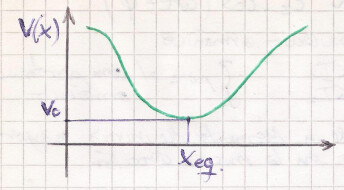
\includegraphics[scale=0.5]{images/fig_mc_oscil_1.jpg}

en un potencial $V(x)$ con un mínimo, es decir que cumple 
\[
	\dtot{V(x)}{x} = 0 ,\dtot[2]{V(x)}{x} > 0
\]
para algún $x_{eq}$, en la expresión de la energía
\be
	E = \frac 1 2 m \dot{x}^2 + V(x),
	\label{energia_1d}
\ee
se aproxima el potencial según\footnote{Nótese que esta es la expansión de Taylor en la cual el término lineal 
está justamente ausente porque la derivada primera en el punto es nula.}
\be
	V(x) \approx V_0 + \frac{1}{2} \left.\dtot[2]{V(x)}{x}\right|_{x_{eq}} (x-x_{eq})^2,
	\label{potencial_aproximado}
\ee
y si definimos $ k \equiv d^2V/dx^2|_{x_{eq}} $ se llega a 
\[
	E = \frac 1 2 m \dot{x}^2 + V_0 + \frac{1}{2} k (x-x_{eq})^2, 
\]
que derivada con respecto al tiempo resulta en 
\[
	m\ddot{x} + k (x-x_{eq}) = 0,
\]
la cual no es otra cosa que una ecuación de oscilador armónico, cuya solución general es
\[
	x(t) = A \cos (\omega t + \varphi ),
\]
donde $ \omega =  \sqrt{ k / m } $ y $ \varphi $ está asociada a la energía $E$. Ver Apéndice X para la resolución
de oscilador armónico.
\notamargen{Un apéndice más: oscilador armónico con término no homogéneo (usar 76R carpeta). Acá habría que llegar a despejar quién es
$\varphi$.}

El problema físico tiene dos constantes aunque la resolución presenta cuatro (dos complejos, con parte real e imaginaria).

\subsection{Varias variables}

En el caso de un potencial $V(\vb{x}_1, ...,\vb{x}_n)$ hay que hallar las raíces del mismo y luego desarrollar en torno a los puntos
de equilibrio. Se empieza desde 
\[
	\dpare{V}{\vb{x}}{x_{eq}} = 0,
\]
y habría que desarrollar 
\[
	V( \vb{x}_1, ...,\vb{x}_n ) = V( \vb{x}_1, ...,\vb{x}_n ) + 
	\frac 1 2 \sum_{i,j} \dparcru{V}{\vb{x}_i}{\vb{x}_j}(\vb{x}-\vb{x}_i)(\vb{x}-\vb{x}_j)
\]

No obstante, el problema se puede enfocar mejor en términos de las coordenadas generalizadas. Entonces, el potencial es
\[
	V(q_1,...,q_n) \approx V(q_1^0,...,q_n^0) + \sum_{i=1}^n \left. \dpar{V}{q_i} \right|_{q_i^0} (q_i - q_i^0)
		+ \frac{1}{2} \sum_{i,j=1}^n \left. \dparcru{V}{q_j}{q_i}\right|_{q_i^0}(q_i -q_i^0)(q_j -q_i^0)
\]
y la energía cinética,
\[
	T(q_1,...,q_n,\dot{q}_1,...,\dot{q}_n) \approx \frac{1}{2} \left( m(q_1^0,...,q_n^0) + \sum_{i=1}^n 
				\left. \dpar{m}{q_i} \right|_{q_i^0} (q_i - q_i^0) + ... \right) \sum_{i,j}^n \dot{q}_i\dot{q}_j
\]
[Esta expresión hay que revisarla y reubicarla!]

La energía cinética es 
\[
	T = \frac 1 2 \sum_{i,j} m_{ij}(q_1,...,q_n) \dot{q}_i \dot{q}_j
\]
donde $m_{ij}$ son los coeficientes de las coordenadas generalizadas y se desarrollarán en serie en torno al equilibrio (caracterizado
por un supraíndice $0$), es decir,
\[
	m_{ij} \approx m_{ij}( q_i^0, ..., q_n^0 ) + \sum_k \dpare{ m_{ij} }{ q_k }{q^0}( q_k - q_k^0 )
\]


Haciendo la aproximación consistente resulta 
\[
	\Lag = T - V = - \frac{1}{2} \sum_{i,j}^n \left. \dparcru{V}{q_j}{q_i}\right|_{q_i^0}(\eta_i)(\eta_j) +
		\frac{1}{2} \sum_{i,j}^n \left. m_{ij}\right|_{q_i^0} \dot{\eta}_i \dot{\eta}_j
\]
con $V_{ij} \equiv \partial^2 V / ( \partial q_i \partial q_j ) |_{q_i^0}, m_{ij} = m_{ij}|_{q_i^0}$ simétricos 
y donde se ha definido $\eta_i = q_i - q_i^0$. Notemos que $\dot{q}_i = \dot{\eta}_i $.
Con esta nomenclatura puede escribirse
\[
	\Lag = \frac{1}{2} \sum_{i,j=1}^n m_{ij} \dot{\eta}_i \dot{\eta}_j - \frac{1}{2} \sum_{i,j=1}^n V_{ij} \eta_i \eta_j
\]
siendo ambas sumatorias formas bilineales cuadráticas reales y definidas positivas. Matricialmente,
\[
	\Lag = \frac{1}{2} \dot{\vb{\eta}}^t \mathbb{T} \dot{\vb{\eta}} - \frac{1}{2} \dot{\vb{\eta}}^t \mathbb{V} \dot{\vb{\eta}}
\]
y si ahora evaluamos las ecuaciones de Euler-Lagrange para este formalismo resulta que 
\[
	\frac{d}{dt}\left( \dpar{\Lag}{\dot{\eta}_k} \right) - \dpar{\Lag}{\eta_k} = 
		\frac{d}{dt} \left( \frac{1}{2} \sum_{i,j=1}^n m_{ij} \frac{d}{d\dot{\eta}_k}(\dot{\eta}_i \dot{\eta}_j) \right) - 
		\frac{1}{2} \sum_{i,j=1}^n V_{ij} \frac{d}{d\eta_k} (\eta_i \eta_j) = 0
\]
son $n$ ecuaciones diferenciales de Euler, 
\[
	\sum_{j=1}^n m_{kj} \ddot{\eta}_j + V_{kj} \eta_j = 0 \qquad k=(1,...,n).
\]

Se propone como solución 
\[
	\eta_j(t)  = A_j e^{i\omega t}
\]
tomando al final del proceso $\Re\{A_j e^{i\omega t}\}$ como solución física. Esta elección lleva a
\[
	\sum_{j=1}^n ( - \omega^2 m_{kj} + V_{kj} ) A_j = 0
\]
que equivale a
\[
	(\mathbb{V} -\omega^2\mathbb{T})\vb{A} = 0
\]
que no es otra cosa que un problema de autovalores y autovectores generalizado. Necesito
\[
	\left| \mathbb{V} -\omega^2\mathbb{T} \right| = 0
\]
siendo $\omega^2_1, ...,\omega^2_n$ autofrecuencias con $\omega^2_s \in \mathbb{R}$ y $\omega^2_s \geq 0$.

Entonces, dado un $V=V(q_i)$ puede ser más fácil obtener explícitamente la serie de Taylor con 
$\partial^2 V/ \partial q_i \partial q_j |_{q_i^0}$ o bien cambiar variable $\eta = q_i - q_i^0$ y quedarse
con los términos cuadráticos en $\eta_i \eta_j$. Para la energía cinética $T=T(q,\dot{q})$ puede ser más
fácil evaluar $m_{ij}(q_i)|_{q_i^0}$ y quedarnos con los términos cuadráticos en $\dot{\eta}_i \dot{\eta}_j$.

\[
	\eta_j^s = A_j^s e^{i\omega_s t}	 \qquad s=1,...,N
\]
Vectorialmente es 
\[
	\vb{\eta}^s = \vb{A}_j^s e^{i\omega_s t} = \begin{pmatrix}
	                A_1 e^{i\omega_s t} \\
	                A_2 e^{i\omega_s t} \\
	                ... \\
	                A_N e^{i\omega_s t} \\
	               \end{pmatrix}
\]
para la frecuencia $\omega_s$, siendo cada uno un grado de libertad moviéndose con frecuencia $\omega_s$.

Luego, es
\[
	\vb{\eta}_{tot} = c_1 \vb{\eta}^1 + c_2 \vb{\eta}^2 + ... + c_N \vb{\eta}^N
\]
\[
	\vb{\eta}_{tot} = \begin{pmatrix}
				\eta_1 \\
				\eta_2 \\
				... \\
				\eta_n 
	                  \end{pmatrix}
	                 = \begin{pmatrix}
				c_1 A_1^1 e^{i\omega t} + c_2 A_1^2 e^{i\omega t} + ... + c_n A_1^n e^{i\omega t} \\
				c_1 A_2^1 e^{i\omega t} + c_2 A_2^2 e^{i\omega t} + ... + c_n A_2^n e^{i\omega t} \\
				... \\
				c_1 A_n^1 e^{i\omega t} + c_2 A_n^2 e^{i\omega t} + ... + c_n A_n^n e^{i\omega t}
	                  \end{pmatrix}
\]
entonces $\vb{A}^s$ es un modo normal de frecuencia $s$.
\[
	\vb{A}^s = \begin{pmatrix}
	            A_1^s \\
	            A_2^s \\
	            ... \\
	            A_n^s
	           \end{pmatrix}
	           e^{i\theta_0}
\]

La solución total ($j$ es el grado de libertad) se puede escribir 
\[
	\eta_j(t) = \sum_{s=1}^N c_s A_j^s e^{i\omega_s t}
\]
\[
	\vb{\eta}(t) = \sum_{s=1}^N c_s \vb{A}^s e^{i\omega_s t}
\]
y finalmente 
\[
	\vb{\eta}(t) = \Re \left\{ \sum_{s=1}^N c_s \vb{A}^s e^{i\omega_s t} \right\}
\]

Matricialmente,
\[
	\vb{A}^\dagger \mathbb{T} \vb{A} = 1
\]
siendo el $\dagger$ el traspuesto conjugado. Se pide que la norma (en la métrica dada por $\mathbb{T}$ de la unidad)
\[
	A^t \mathbb{T} A = \mathbb{1}
\]
lo cual significa que $A$ diagonaliza a $\mathbb{T}$, siendo 
\[
	A = \begin{pmatrix}
	     A_1^1 & A_1^2 & ... & A_1^n \\
	     A_2^1 & ... \\
	     A_n^1 & A_n^2 & ... & A_n^n 
	    \end{pmatrix}
\]
la matriz modal donde sus columnas son autovectores.

\[
	(\mathbb{V} - \omega^2 \mathbb{T})\vb{A} = 0
\]
interpolando a la matriz 
\[
	A^t \mathbb{V} A = \omega^2 A^t \mathbb{T} A= \omega^2 \mathbb{1}
\]
y sea ahora el siguiente cambio de coordenadas
\[
	\vb{\eta} = A \vb{\xi}
\]
tal que 
\[
	A^{n\times n} \xi^{n\times 1} \qquad \qquad  (A \vb{\xi} )^t = {\xi^t}^{1 \times n} {A^t}^{n \times n}
\]
y que se llaman coordenadas normales.

\[
	\Lag = \frac{1}{2} \dot{\vb{\eta}}^t \mathbb{T} \dot{\vb{\eta}} - \frac{1}{2} \dot{\vb{\eta}}^t \mathbb{V} \dot{\vb{\eta}}
\]
\[
	\Lag = \frac{1}{2} A^t\dot{\vb{\xi}}^t \mathbb{T} A \dot{\vb{\xi}} - \frac{1}{2} A^t\dot{\vb{\xi}}^t \mathbb{V} 
\dot{\vb{\xi}}
\]
\[
	\Lag = \frac{1}{2} \dot{\vb{\xi}}^t \mathbb{1} \dot{\vb{\xi}} - \frac{1}{2} \dot{\vb{\xi}}^t \omega^2 \mathbb{1} \dot{\vb{\xi}}
\]

\[
	\Lag = \frac{1}{2} \sum_i \dot{\vb{\xi}}_i^2 - \frac{1}{2} \sum_i \vb{\xi}_i^2 \omega^2_i 
\]
\[
	\frac{d}{dt}\left( \dpar{\Lag}{\dot{\xi}_i} \right)- \dpar{\Lag}{\xi_i} = \sum_i \ddot{\xi}_i + \omega^2_i \xi_i = 0 
\]
y son $N$ ecuaciones de Euler-Lagrange.
\[
	\sum_i ( -\omega^2 + \omega^2_i ) A_i = 0
\]
de modo que si $\omega^2 = \omega^2_i$ entonces
\[
	\xi_i = C_i e^{i\omega_i t}
\]

Digamos que en coordenadas normales
\[
	\xi_j = C_j e^{i \omega_j t}
\]
grados de libertad en $\xi$ (un grado de libertad es una $\omega$) y se desacoplan los grados de libertad
en lo que hace a $\omega_s$.
Por otro lado,
\[
	\eta_j = \sum_{s=1}^N c_s A_j^s e^{i \omega_j t}
\]
grados de libertad en $\eta$, un grado de libertad entonces es combinación lineal de todas las $\omega$.

Si $\omega=0$ es 
\[
	\xi_j = At + B 
\]
\[
	\eta_j = \sum_{s=1}^{N-1} c_s A_j^s e^{i \omega_j t} + A_j(Gt + D)
\]
siendo el último término asociado a la $\omega=0$.
Para volver atrás es 
\[
	A^{\dagger} \mathbb{T} A = \mathbb{1}
\]
y entonces 
\[
	A^{\dagger} \mathbb{T} \vb{\eta} = A^{\dagger} \mathbb{T} A \vb{\xi}  
\]
\[
	A^{\dagger} \mathbb{T} \vb{\eta} = \mathbb{1} \xi
\]
coordenadas normales en función de las de desplazamiento.

En conclusión podemos decir varias cosas,
\begin{itemize}
 \item Las frecuencias nulas están asociadas a momentos conservados.
 \item En coordenadas normales cada grado de libertad oscial con una frecuencia única (son $N$
	osciladores independientes)
 \item Las amplitudes cumplen
 \[ \vb{A}^s =
 \begin{pmatrix}
  a_1^s e^{i \phi_s} \\
  a_2^s e^{i \phi_s} \\
  ... \\
  a_n^s e^{i \phi_s}
 \end{pmatrix}
 \]
 donde tienen la misma fase los $A_j^s$ para toda frecuencia $\omega_s$
 \item Los modos normales pueden excitarse por separado (son ortogonales).
 \item Frecuencias iguales generarán modos normales que son físicamente los
 mismos. Son generados por la simetría del problema.
 \[
	\vb{A} = a_1(v_1) + a_2(v_2)
 \]
 si por ejemplo generan dos autovectores de esta forma.
\end{itemize}


% =================================================================================================
\section{Oscilaciones viscosas}
% =================================================================================================

\[
	\sum_j m_{ij} \ddot{\eta}_j + V_{ij}\eta_j + B_{ij}\dot{\eta}_j = 0
\]
no se puede convertir en osciladores independientes.
\[
	det\left\{ \mathbb{V} + \omega^2 \mathbb{T} + \omega \mathbb{B}\right\} = 0
\]






% \bibliographystyle{CBFT-apa-good}	% (uses file "apa-good.bst")
% \bibliography{CBFT.Referencias} % La base de datos bibliográfica

\end{document}
